We present some examples that illustrates the use of Qlang in solving quantum computing problems.

\subsection { Solving Quantum Computation Problem}
\subsubsection{Problem1}
Evaluate the following expressions: a. $(H \otimes X) \ket{00}$ b. $\dotproduct[101,000]$ c. $\bra{01} H \otimes H \ket{01} $
\begin{lstlisting}
	
def pseudo = evaluate (){
		
	# a quit type declaration follows dirac notation
	qub mat0 = |00>;
		
	# Both X and H are constant with type mat and
	# @ corresponds to tensor product.
	mat HX = H @ X;
		
	pseudo = HX * mat0;
}
	
\end{lstlisting}

\subsubsection{Problem 2}
Find the matrix corresponding to the quantum circuit:
\begin{figure}[h!]
\begin{center}
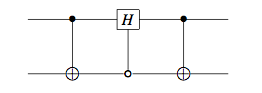
\includegraphics{ref/circuit1}
\end{center}
\caption{ Quantum Circuit implementing series of control gates\label{cir1}}
\end{figure}

\begin{lstlisting}
def circuitMat = findMatrix (){
	
	# all basis qubit in 2 dimension
	qub mat0=|00>;
	qub mat1=|01>;
	qub mat2=|10>;
	qub mat3=|11>;
	
	# controlled not matrix	
	mat CNOT = [1,0,0,0:0,1,0,0:0,0,0,1:0,0,1,0]
	
	#controlled hadmard matrix
	mat HNOT = [1/sqrt(2),0,0,1/sqrt(2):0,1,0,0:1/sqrt(2),0,1,-1/sqrt(2):0,0,0,0]
	#composition of control gates
	mat allGates = CNOT * HNOT * CNOT
	
	# Matrix corresponding to the circuit	
	circuitMat =[allGates*mat0:allGates*mat1:allGates*mat2:allGates*mat3]
		
}
\end{lstlisting}
\subsubsection{Problem 3}
Consider the circuit and show the probabilities of outcome 0 where $\ket{\Psi_{in}} = \ket{1}$
\begin{figure}[h!]
\begin{center}
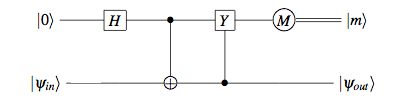
\includegraphics{ref/circuit2}
\end{center}
\caption{ Quantum Circuit\label{cir1}}
\end{figure}

\begin{lstlisting}
def probability = outcomeZero(){
	
	# top and bottom qubits
	qub top = |0>;
	qub bottom = |1>;
	
	# Applying H on top qubit 
	mat output = (H @ I) * (top @ bottom);
	
	# Controlled Not operator
	mat CNOT = [I, [0,0:0,0]: [0,0:0,0], X];
	
	# Controlled Y operator
	mat CY = [Y,[0,0:0,0]:[0,0:0,0], I];
	
	# Applying Control Operators
	output = (CY)*(CNOT)*output
	
	# Applying measurement operator on top qubit |0> <0|
	mat M = (|0>*<0| @ I)
	
	# state after applying measurement operator on top qubit
	outcome = M * output;
	
	#probability of outcome
	probability = norm(outcome);
	
}
\end{lstlisting}

\subsection{ Simulation of Quantum Algorithm}

\subsubsection{Deutsch Jozsa Algorithm}
\begin{lstlisting}

def outcome = deutschJozsa(qub top, mat U){
		
	# in corresponds to the qubit in top register
	# input is the tensor product of top register and bottom register
	mat input=  top @ |1>;
		
	# application of Hadamard gate on both top and bottom inputs
	input = (H @ H)*input;
		
	# application of U gate on the above result
	input = U * input;
		
	# application of Hadamard gate on the top register
	input = (H @ I)*input;
		
	# application of measurement operator on the top register
	# top * Adj (top) corresponds to the Measurement operator
		
	input=(top*Adj(top)@ I)*input;
		
	#after the measurement is applied, check if the input is 0 or not
	if (input == 0){
		#probability of outcome 0 is 0
		outcome = 0;
	}
	else{
		# probability of outcome 0 is 1
		outcome = 1;
	}
}
	
\end{lstlisting}

\subsubsection {Grover's Search Algorithm}

\begin{figure}[h!]
\begin{center}
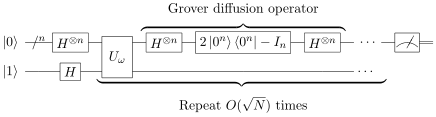
\includegraphics{ref/grover}
\end{center}
\caption{ Grover Algorithm Circuit 
\label{fig:grover}}
\end{figure}

\begin{lstlisting}

def result = grover (quit top, int x0){
	# returns the probability to find x0 for a function f such that f(x0)=1
	# x0 can be x0=0,1,?,2^n-1
	# this is a special case where n=1
	
	# qubit in the bottom register
	qub bottom = |1>;
	
	# tensor product of top and bottom qubit
	mat input = top @ bottom;
	
	#application of Hadamard
	input = (H @ H) * input;
	
	#define S
	mat S = [1,0:0-1]
	
	# k : number of time grover operator is applied
	# for n > 1 k=ceil((pi*2^(n/2))/4);
	int k = 1;
	
	# define O operator  such that O|x>|q>=|x>|q mod f(x)> or O|x>=(-1)f(x)|x> 
	# for n > 1 O = I(2^(n1+1));
	mat O = I;
	O(x0+1, x0+1) = -1;
	
	# Grover iteration matrix
	mat GO = (G*O)^k;
	
	# After application of Grover iteration matrix
	mat output = GO * input;
	
	result = (H @ H)* output;
	
}

\end{lstlisting}
